\subsection{Results}\label{ssec:M2:results}


\subsubsection{Electron fraction} \label{sssec:M2:results:electron_fraction}
The evolution of the electron fraction \note{(mention neutral in general)} with time is shown in \figref{fig:M2:results:decoupling_compare_Xe_peebles_saha}. Here, we have included the solution obtained through the Saha equation alone for comparison. In the figure we also show the time periods when recombination occurs according to the two solutions. We see that the Peebles equation predicts the production of neutral Hydrogen to take much longer time than the Saha equation. Recombination therefore occurs at a much lower temperature than the binding energy of Hydrogen, as expected. Towards $x=0$ the Peebles equation give $\Xe\ll1$, but we never reach $\Xe=0$ entirely, compared to the Saha equation where $\Xe=0$ is eventually reached for sufficiently high values of $x$. 

\begin{figure}[ht!]
    \includefig{decoupling_compare_Xe_peebles_saha}
    \caption{Free electron fraction computed from the Saha equation only (dashed green curve) and from the Peebles equation (solid blue curve), where the Saha equation was used at early times, until $\Xe<0.99$. The decoupling time, i.e. when $\tau=1$, is shown for both the Saha solution (dotted red curve), and for the Peebles solution (dotted black curve).}
    \label{fig:M2:results:decoupling_compare_Xe_peebles_saha}
\end{figure}

\subsubsection{Optical depth and visibility function} \label{sssec:M2:results:optical_depth_and_visibility_function}
\begin{figure}[ht!]
    \includefig{tau_plot}
    \caption{The optical depth, $\tau(x)$ and its two first derivatives with respect to $x$.}
    \label{fig:M2:results:tau_plot}
\end{figure}


\begin{figure}[ht!]
    % 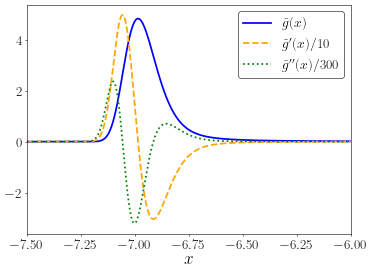
\includegraphics[width=\linewidth]{TEMPg_plot.png}
    \includefig{g_plot}
    \caption{The visibility function, $\gx$ (solid curve), and its derivatives, $\g'(x)/10$ (dashed curve) and $\g''(x)/300$ (dotted curve). The derivatives have been scaled in order to view them all in the same plot.}
    \label{fig:M2:results:g_plot}
\end{figure}

\subsubsection{Times of recombination and decoupling} \label{sssec:M2:results:times_of_recombination_and_decoupling}
The period of recombination and decoupling, as computed from the Peebles equation, is given in table \ref{tab:M2:results:rec_and_dec_time_table_Peebles}. For the decoupling, we also include the value of $x$ when $\g$ is at maximum.

\tablesMilestoneTwo{rec_and_dec_time_table_Peebles.tex}

\tablesMilestoneTwo{rec_and_dec_time_table_Saha.tex}
